
\chapter{Appendix}
\begin{appendices}

    \begin{figure}[H]
        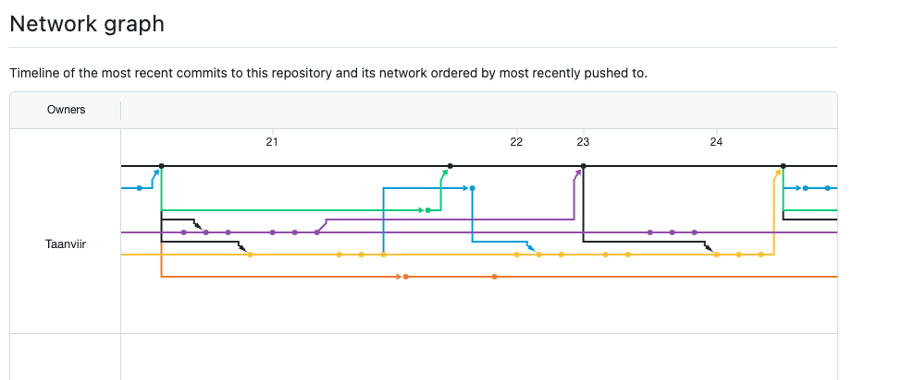
\includegraphics[width=1\linewidth]{./images/network-graph.png}
        \caption*{Network graph of GitHub, representing the main branch (black), fixes on the game (green), improvement of design of the pages (purple), and features of user management (yellow and blue).}
        \label{fig:network-grahp}
    \end{figure}
    
    \begin{figure}[H]
        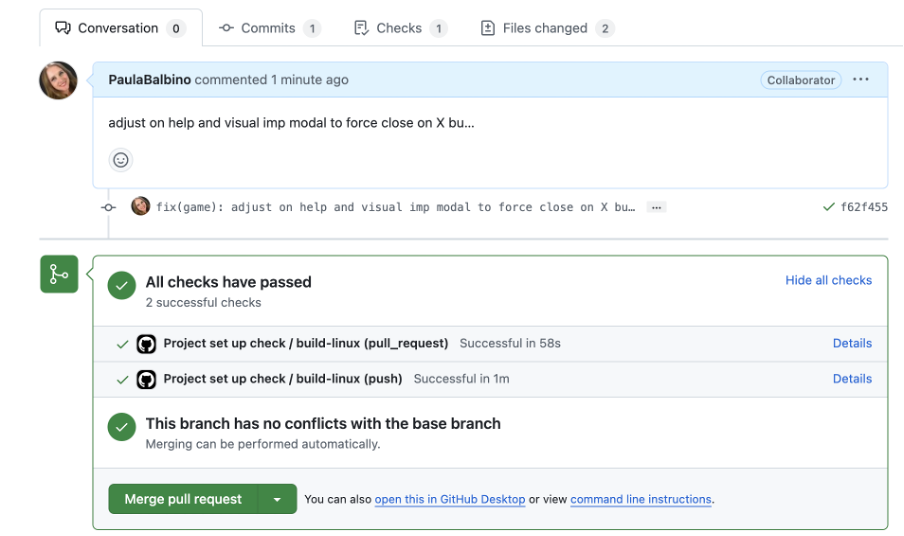
\includegraphics[width=1.0\linewidth]{images/ci-cd.png}
        \caption*{Example of CI/CD integration on GitHub.}
        \label{fig:ci-cd}
    \end{figure}
    
    \begin{figure}[H]
        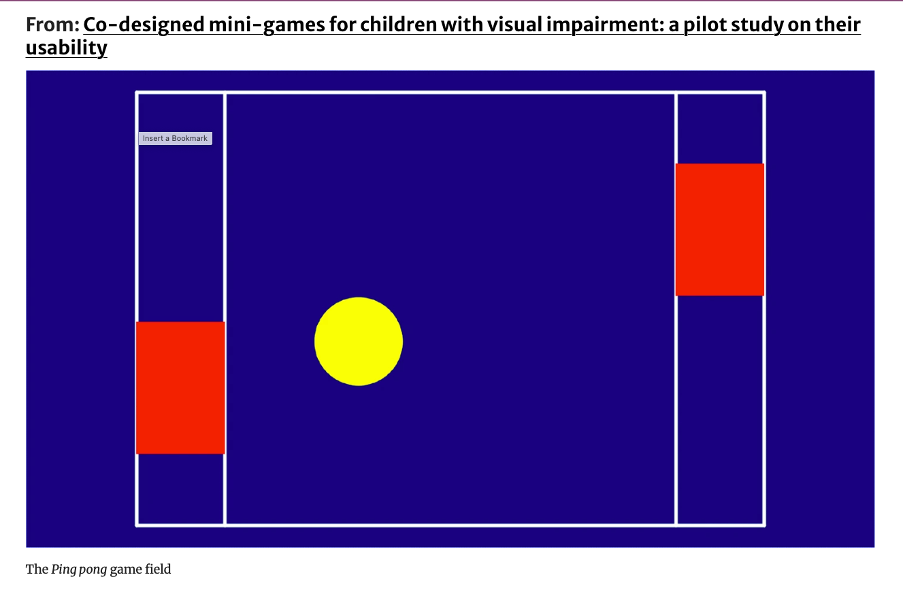
\includegraphics[width=1.0\linewidth]{images/vi-impairment.png}
        \caption*{The visual impairment mode of the project was inspired by the study Co-designed mini-games for children with visual impairment: A pilot study on their usability by Battistin et al. (2022), which explored accessible game design principles tailored for visually impaired children to enhance usability and engagement.}
        \label{fig:impairment}
    \end{figure}
    
\end{appendices}